\documentclass{beamer}
\usepackage{amsmath,amssymb,latexsym,array,fancyheadings,mathdots}
\usepackage{algorithm,algorithmic}
\usepackage{hyperref}
\usepackage{color}
\usepackage{tabularx}
\usepackage[all]{xy}
\usepackage{qtree}
\usepackage{gitinfo2}

%% RCS
%\usepackage{rcs}

%% Colors
\definecolor{darkgreen}{rgb}{0,.4,0}
\definecolor{darkred}{rgb}{.5,0,0}
\definecolor{darkmagenta}{rgb}{.5,0,.5}
\definecolor{orange}{rgb}{1,.5,0}
\definecolor{lightblue}{rgb}{0.122,0.016,0.855}
\definecolor{darkocre}{rgb}{0.471,0.298,0.008}

\usetheme{default}

%% New Theorems
\newtheorem{thm}{Theorem}
\newtheorem{exm}[thm]{Example}
\newtheorem{cor}[thm]{Corollary}
\newtheorem{propo}[thm]{Proposition}
\newtheorem{lem}[thm]{Lemma}
\newtheorem{clm}[thm]{Claim}
\newtheorem{exr}[thm]{Exercise}
\newtheorem{dfn}[thm]{Definition}

%% New commands
\newcommand{\classfont}{\mathsf}
\newcommand{\ATM}{\classfont{A}_{\mathrm{TM}}}
\newcommand{\MTF}{\mathrm{MTF}}
\newcommand{\OPT}{\mathrm{OPT}}
\newcommand{\ALG}{\mathrm{ALG}}
\newcommand{\ALGNAIVE}{\mathrm{ALG}_{\text{na{\"\i}ve}}}
\newcommand{\LRU}{\mathrm{LRU}}
\newcommand{\FIFO}{\mathrm{FIFO}}
\newcommand{\FWF}{\mathrm{FWF}}
\newcommand{\LFD}{\mathrm{LFD}}
\newcommand{\true}{\mathsf{T}}
\newcommand{\false}{\mathsf{F}}
\newcommand{\also}{\wedge}
\newcommand{\lra}{\leftrightarrow}
\newcommand{\tc}{\textcolor}
\newcommand{\df}[1]{\textcolor{red}{\em #1}}
\newcommand{\highlight}[1]{\textcolor{orange}{\em #1}}
\newcommand{\hl}[1]{\textcolor{blue}{\em #1}}
\newcommand{\amp}{\texttt{\&}}
\newcommand{\hsh}{\texttt{\#}}
\newcommand{\ra}{\rightarrow}
\newcommand{\longra}{\longrightarrow}
\newcommand{\Ra}{\Rightarrow}
\newcommand{\rab}{{\rightarrow_\beta}}
\newcommand{\srab}{{\rightarrow^*_\beta}}
\newcommand{\aeq}{{=_\alpha}}
\newcommand{\order}{\mathrm{order}}
\newcommand{\rem}{\mathrm{rem}}
\newcommand{\IP}{\mathbf{IP}}
\newcommand{\PSPACE}{\mathbf{PSPACE}}
\newcommand{\thevalue}{\text{value}}
\newcommand{\pol}[1]{\mathbf{#1}}
\newcommand{\enc}{\text{Enc}}
\newcommand{\xor}{\oplus}
\newcommand{\zo}{\{0,1\}}
\newcommand{\SOPT}{S_{\mathrm{opt}}}
\newcommand{\la}{\leftarrow}
\newcommand{\myurl}[1]{\textcolor{darkgreen}{\url{#1}}}
\newcommand{\myhref}[2]{\textcolor{darkgreen}{\href{#1}{#2}}}
\newcommand{\qaccept}{q_{\mathrm{accept}}}
\newcommand{\qreject}{q_{\mathrm{reject}}}
\newcommand{\opt}{\text{\sc Opt}}
\newcommand{\tr}{\mathrm{tr}}
\newcommand{\csanky}{p^{\textsc{csanky}}}
\newcommand{\berk}{p^{\textsc{berk}}}

%% Algorithms package customization
\renewcommand{\algorithmicrequire}{\textbf{Pre-condition:}} 
\renewcommand{\algorithmicensure}{\textbf{Post-condition:}} 
\algsetup{indent=3em}

\input{prooftree}

%% including/excluding pauses
\newcommand{\ifpause}{\iftrue} % for including pauses
%\newcommand{\ifpause}{\iffalse} % for excluding pauses

%% 2nd or 3rd edition
\newif\ifthird
\thirdtrue
%\thirdfalse

%disables usefoottemplate
\setbeamertemplate{navigation symbols}{}
%\setbeamertemplate{footline}% 
%{\strut\quad\tiny 
%\begin{minipage}{3cm}
%Cryptography - Michael Soltys
%\today\ {\tt v\RCSRevision}
%\end{minipage}\hfill
%\insertsection\
%- \insertframenumber/\inserttotalframenumber\quad\strut}

\newcommand{\mytitle}{Preliminaries}
\newcommand{\mychpnr}{1}
%% Title page contents
\title{Intro to Analysis of Algorithms \\ \mytitle \\  Chapter \mychpnr}
\author{Michael Soltys}
\date{\textcolor{darkgreen}{\tiny\tt 
[ {\bf Git} Date:\gitAuthorDate\ 
Hash:\gitAbbrevHash\ 
Ed:\ifthird
3rd
\else
2nd
\fi]}}
\institute{CSU Channel Islands}

\setbeamertemplate{footline}{
  \colorbox{white}{\color{black}\tt
     \begin{tabularx}{0.97\textwidth}{XXX}
          IAA Chp \mychpnr\ - Michael Soltys \copyright & 
          \hfill\today\ (\gitAbbrevHash; \ifthird ed3\else ed2\fi)
					\hfill\phantom{.} & 
          \hfill\insertsection\ - \insertframenumber/\inserttotalframenumber \\
      \end{tabularx}}}

\begin{document}

\mode<presentation>
{
}

\parskip 8pt

\section{Introduction}

\begin{frame}
\titlepage
\end{frame}


\begin{frame}
\begin{enumerate}
\item Precondition
\item Postcondition
\item Termination
\item Partial Correctness
\item Correctness (Full Correctness)
\end{enumerate}
\end{frame}

\begin{frame}
Boolean connectives: $\wedge$\label{wedge} is
``and,'' $\vee$ is ``or'' and $\neg$ is ``not.''  

We also use $\ra$ as
Boolean implication, i.e., $x\ra y$ is logically equivalent to $\neg
x\vee y$, and  
$\leftrightarrow$ is Boolean equivalence,
and $\alpha\lra\beta$ expresses
$((\alpha\ra\beta)\wedge(\beta\ra\alpha))$. 

$\forall$ is the
``for-all'' universal quantifier, and $\exists$ is the ``there
exists'' existential quantifier.

We use ``$\Rightarrow$'' to abbreviate the word
``implies,'' i.e., $2|x\Rightarrow x$ is even, while
``$\not\Rightarrow$'' abbreviates ``does not imply.''
\end{frame}

\begin{frame}
Partial Correctness:
\begin{equation}\tag{\ifthird 1.1\else 1.3\fi}
(\forall I\in\mathcal{I}_A)
[(\alpha_A(I)\wedge\exists
O(O=A(I)))\ra\beta_A(A(I))]
\end{equation}

How to modify it to express full correctness?
\ifthird
(Problem 1.1) 
\else
% Problem 1.1 does not exist in 2nd ed, so nothing
\fi
\end{frame}

\section{Division}

\begin{frame}
{\bf Division Algorithm (A\ifthird 1.1\else 1.1\fi)}

\begin{algorithmic}[1]
\REQUIRE $x\geq 0 \also y>0 \also x,y\in\mathbb{N}$
\STATE $q\leftarrow 0$
\STATE $r\leftarrow x$
\WHILE{$y\le r$}
       \STATE $r\leftarrow r-y$
       \STATE $q\leftarrow q+1$
\ENDWHILE
\RETURN $q,r$
\ENSURE $x=(q\cdot y)+r \also 0\le r<y$
\end{algorithmic}

\end{frame}

\begin{frame}

Loop invariant:

\begin{equation}\tag{\ifthird 1.2\else 1.4\fi}
x=(q\cdot y)+r \also r\geq 0.
\end{equation}

Show that it holds true after each iteration of the loop:

Basis case (i.e., zero iterations of the loop---we are just before
line~3 of the algorithm): $q=0,r=x$, so
$x=(q\cdot y)+r$ and since $x\geq 0$ and $r=x$, $r\geq 0$.  
\end{frame}

\begin{frame}

Induction step: suppose $x=(q\cdot y)+r\also r\geq 0$ and we go once
more through the loop. 

Let $q',r'$ be the new values of $q,r$,
respectively (computed in lines 4 and 5 of the algorithm).  

Since we
executed the loop one more time it follows that $y\leq r$ (this is the
condition checked for in line~3 of the algorithm), and
since $r'=r-y$, we have that $r'\geq 0$.  Thus,
$$
x=(q\cdot y)+r=((q+1)\cdot y)+(r-y)=(q'\cdot y)+r',
$$ 
and so $q',r'$ still satisfy the loop invariant.
\end{frame}

\begin{frame}
{Partial Correctness}

Now we use the loop invariant to show that (if the algorithm
terminates) the post-condition of the
division algorithm holds, {\em if} the pre-condition holds.  

This is
very easy in this case since the loop ends when it is no longer true
that $y\leq r$, i.e., when it is true that $r<y$.

On the other hand, we proved already that loop invariant holds after
each iteration, in particular the last one. Putting it all together we
get the post-condition.
\end{frame}

\begin{frame}
{Termination}

To show termination we use the least number principle (LNP).  

We need
to relate some non-negative monotone decreasing sequence to the
algorithm; just consider $r_0,r_1,r_2,\ldots$, where $r_0=x$, and
$r_i$ is the value of $r$ after the $i$-th iteration.  

Note that
$r_{i+1}=r_i-y$.  

First, $r_i\ge 0$, because the algorithm enters the
while loop only if $y\le r$, and second, $r_{i+1}<r_i$, since $y>0$.

By LNP such a sequence ``cannot go on for ever,'' (in the sense that
the set $\{r_i|i=0,1,2,\ldots\}$ is a subset of the natural numbers,
and so it has a least element), and so the algorithm must terminate.
\end{frame}

\begin{frame}

\ifthird
{\bf Problem 1.3}
\else
% Problem not in ed2
\fi

What is the running time of the algorithm? That is, how many steps
does it take to terminate? Assume that assignments (lines 1 and 2),
and arithmetical operations (lines 4 and 5) as well as testing
``$\le$'' (line 3) all take one step.
\end{frame}

\section{Euclid}

\begin{frame}
{\bf Euclid's Algorithm (A\ifthird 1.2\else 1.2\fi)}

Given two positive integers $a$ and $b$, their 
{\em greatest common divisor},
denoted as $\gcd(a,b)$, is the largest positive integer
that divides them both.

\begin{algorithmic}[1]
\REQUIRE $a>0 \also b>0 \also a,b\in\mathbb{Z}$ 
\STATE $m\leftarrow a$ ; $n\leftarrow b$ ; $r\leftarrow\rem(m,n)$
\WHILE{$(r>0)$}
\STATE $m\leftarrow n$ ; $n\leftarrow r$ ; $r\leftarrow\rem(m,n)$
\ENDWHILE
\RETURN $n$
\ENSURE $n=\gcd(a,b)$
\end{algorithmic}
\end{frame}

\begin{frame}
Unlike division, Euclid's algorithm is very fast.

This is very important, as it is one of the building blocks of
Cryptography; see Problem~\ifthird 6.10\else 6.9\fi, % REFERENCE
which leads to the correctness of the
Rabin-Miller algorithm.

The Rabin-Miller algorithm (Algorithm 6.3) % REFERENCE
for primality testing is what makes Publick Key Crypto such as
Diffie-Hellman, El Gamal, RSA, etc., possible.
\end{frame}

\begin{frame}
Loop Invariant:
\begin{equation}\tag{1.3}
m>0,n>0\text{ and }
\gcd(m,n)=\gcd(a,b)
\end{equation}

Basis Case: $m=a>0$ and $n=b>0$ and so loop invariant holds

Induction Step: suppose $m,n>0$ and 
$\gcd(a,b)=\gcd(m,n)$, and we go
through the loop one more time, yielding $m',n'$.  

We want to show
that $\gcd(m,n)=\gcd(m',n')$.  

Note that from line~3 of the
algorithm we see that $m'=n,n'=r=\rem(m,n)$, so in particular
$m',n'>0$,
since if $r=\rem(m,n)$ were zero, the loop
would have terminated (and we are assuming that we are going through
the loop one more time). 
\end{frame}

\begin{frame}
Problem \ifthird 1.6\else 1.18\fi: 
Show that for all $m,n>0$, $\gcd(m,n)=\gcd(n,\rem(m,n))$.

Problem \ifthird 1.7\else 1.19\fi: Show that Euclid's algorithm terminates.

Problem: \ifthird 1.7\else \fi:  what is the complexity of Euclid's algorithm?

{\color{blue}
More challenging problem: Show that for any integer $k\ge 1$, if
$a>b\ge 1$ and $b<F_{k+1}$ (where $F_i$ is the $i$-th Fibonacci
number), then Euclid's algorithm on $a,b$ takes fewer than $k$
iterations of the while loop. (Ignore swaps, or use $2k$ instead.)
}
\end{frame}

\section{Palindromes}

\begin{frame}
{\bf Palindromes (A\ifthird 1.3\else 1.3\fi)}

\colorbox{yellow}{\tt racecar}

\bigskip

\begin{algorithmic}[1]
\REQUIRE $n\geq 1\also A[1\ldots n]$ is a character array
\STATE $i\leftarrow 1$ 
\WHILE{($i\le\lfloor\frac{n}{2}\rfloor$)} 
      \IF{($A[i]\neq A[n-i+1]$)}
          \RETURN $\false$ 
      \ENDIF
\STATE $i\leftarrow i+1$ 
\ENDWHILE
\RETURN $\true$ 
\ENSURE return $\true$ iff $A$ is a palindrome
\end{algorithmic}

\end{frame}

\begin{frame}
Let the loop invariant be: after the $k$-th iteration, $i=k+1$ and for
all $j$ such that $1\le j\le k$, $A[j]=A[n-j+1]$. 

We prove that the
loop invariant holds by induction on~$k$.  

Basis case: before any
iterations take place, i.e., after zero iterations, there are no
$j$'s such that $1\le j\le 0$, so the second part of the loop
invariant is (vacuously) true.  The first part of the loop invariant
holds since $i$ is initially set to~$1$.

Induction step: we know that after $k$ iterations, $A[j]=A[n-j+1]$ for
all $1\le j\le k$; after one more iteration we know that
$A[k+1]=A[n-(k+1)+1]$, so the statement follows for all $1\le j\le
k+1$.  This proves the loop invariant.
\end{frame}

\begin{frame}
Show partial correctness of the palindromes algorithm.

Does it terminate? If yes, what is its complexity?

Other practice problems: \ifthird 1.13,14,15\else 1.25,26,27\fi
\end{frame}

\section{Python strings}

\begin{frame}
{\bf Python String Manipulations}

In is easy to manipulate strings in Python; a segment of a string is
called a {\em slice}\index{Python!string!slice}.  Consider the word
{\tt palindrome}; if we set the variables {\tt s} to this word,

{\tt s = 'palindrome'}

then we can access different slices as follows:

{\tt
print s[0:5]      palin \\
print s[5:10]     drome \\
print s[5:]       drome \\
print s[2:8:2]    lnr
}

where the notation {\tt [i:j]} means the segment of the string
starting from the $i$-th character (and we always start counting at
zero!), to the $j$-th character, including the first but excluding the
last.  
\end{frame}

\begin{frame}
The notation {\tt [i:]} means from the $i$-th character, all
the way to the end, and {\tt [i:j:k]} means starting from the $i$-th
character to the $j$-th (again, not including the $j$-th itself),
taking every $k$-th character.

One way to understand the string delimiters is to write the indices
``in between'' the numbers, as well as at the beginning and at the
end.  For example
$$
{}_{0}
\texttt{p}
{}_{1}
\texttt{a}
{}_{2}
\texttt{l}
{}_{3}
\texttt{i}
{}_{4}
\texttt{n}
{}_{5}
\texttt{d}
{}_{6}
\texttt{r}
{}_{7}
\texttt{o}
{}_{8}
\texttt{m}
{}_{9}
\texttt{e}
{}_{10}
$$
and to notice that a slice {\tt [i:j]} contains all the symbols
between index $i$ and index $j$.
\end{frame}

\begin{frame}
\ifthird Problem 1.12 \else \fi
What is the shortest Python program you can write to test whether the
string $s$ is a palindrome?

\vskip 2cm
Here is a fun problem: on September 11, 2019, we started a ``{\em
palindromic week},'' meaning that the dates (given in the format
\{M,MM\}\{D,DD\}YY) are palindromes: 91119,91219,91319,$\ldots$,91819.
When is the next palindromic week? Will we be so lucky as to live and
experience it?
\end{frame}

\begin{frame}
{\bf Is it obvious when algorithms terminate?}

\begin{algorithmic}
\REQUIRE $a>0$
\STATE $x\longleftarrow a$
\WHILE{last three values of $x$ not $4,2,1$}
	\IF{$x$ is even}
		\STATE $x\longleftarrow x/2$
	\ELSE
		\STATE $x\longleftarrow 3x+1$
	\ENDIF
\ENDWHILE
\end{algorithmic}


\end{frame}

\section{Ranking Algorithms}

\begin{frame}
{\bf Ranking Algorithms}

\begin{itemize}
\item PageRank
\item Stable Marriage
\item Pairwise Comparisons
\end{itemize}
\end{frame}

\begin{frame}
{PageRank}

\begin{enumerate}
\item 1945 article by Vannevar Bush on the ``Memex''
\item 1990s Berners-Lee and hyperlinks (HTML)
\item Huge WWW: how to find a relevant page?
\item Authoritative pages
\end{enumerate}
\end{frame}

\begin{frame}
A web page $X$, and all the pages $T_1,T_2,T_2,\ldots,T_n$ that point
to it.
\begin{center}
\begin{minipage}{6cm}
\xymatrix{
*++[o][F-]{T_1}\ar[rrd] & 
*++[o][F-]{T_2}\ar[rd] & 
*++[o][F-]{T_3}\ar[d] & \ldots & 
*++[o][F-]{T_n}\ar[lld] \\
&& *++[o][F-]{X} &&
}
\end{minipage}
\end{center}
\end{frame}

\begin{frame}
Given a page
$X$, let $\text{C}(X)$ be the number of distinct links that leave $X$, i.e.,
these are links anchored in $X$ that point to a page outside of $X$.

Let $\text{PR}(X)$ be the page rank of $X$. We also employ a paramater
$d$, which we call the {\em damping factor}.

$$
\text{PR}(X)=(1-d)+d\left[
\frac{\text{PR}(T_1)}{\text{C}(T_1)}+
\frac{\text{PR}(T_2)}{\text{C}(T_2)}+\cdots+
\frac{\text{PR}(T_n)}{\text{C}(T_n)}\right].
$$
\end{frame}

\begin{frame}
\begin{center}
\begin{minipage}{6cm}
\xymatrix{
\ar@{}[r]^(.18){}="a"^(.80){}="b" \ar "a";"b" & *++[o][F-]{A}\ar[r] & 
*++[o][F-]{B}\ar[ld]\ar[d]\ar[rd]\ar[r] & 
*++[o][F-]{C}\ar[d] \\
& *++[o][F-]{D}\ar[r] & 
*++[o][F-]{E}\ar[ur] & 
*++[o][F-]{F}\ar@{-} `dr_l `l[ulll] `_r [lllu]
}
\end{minipage}
\end{center}
\end{frame}

\begin{frame}
Using Excel with the following formulas: initially (Stage 0) all get
$1/6$, and then they are computed with:
\begin{tabular}{l}
$\text{PR}(A)=\text{PR}(F)$ \\
$\text{PR}(B)=\text{PR}(A)$ \\
$\text{PR}(C)=\text{PR}(B)/4+\text{PR}(E)$ \\
$\text{PR}(D)=\text{PR}(B)/4$ \\
$\text{PR}(E)=\text{PR}(B)/4+\text{PR}(D)$ \\
$\text{PR}(F)=\text{PR}(B)/4+\text{PR}(C)$ \\
\end{tabular}
\end{frame}

\begin{frame}[fragile]
\begin{verbatim}
Stage	0     1     2     3     4     5     ...   17
----------------------------------------------------
A     0.17  0.17  0.21  0.25  0.29  0.18        0.22
B     0.17  0.17  0.17  0.21  0.25  0.29        0.22
C     0.17  0.21  0.25  0.13  0.14  0.16        0.17
D     0.17  0.04  0.04  0.04  0.05  0.06        0.06
E     0.17  0.21  0.08  0.08  0.09  0.11        0.11
F     0.17  0.21  0.25  0.29  0.18  0.20        0.22
----------------------------------------------------
Total 1.00  1.00  1.00  1.00  1.00  1.00        1.00
\end{verbatim}
\end{frame}

\begin{frame}
{Stable Marriage}

An instance of the {\em stable marriage problem}
of size $n$ consists
of two disjoint finite sets of equal size; a set of {\em boys}
$B=\{b_1,b_2,\ldots,b_n\}$, and a set of {\em girls}
$G=\{g_1,g_2,\ldots,g_n\}$.

Let ``$<_i$'' denote the ranking of boy $b_i$; that is, $g<_ig'$ means
that boy $b_i$ prefers $g$ over $g'$.  

Similarly, ``$<^j$'' denotes
the ranking of girl $g_j$.

Each boy $b_i$ has such a ranking (linear
ordering) $<_i$ of $G$ which reflects his preference for the girls that
he wants to marry.

Similarly each girl $g_j$ has a ranking
(linear ordering) $<^j$ of $B$ which reflects her preference for the
boys she would like to marry.
\end{frame}

\begin{frame}
A {\em matching} (or {\em marriage}) $M$ is a 1-1 correspondence
between $B$ and $G$.  

We say that $b$ and $g$ are {\em partners} in
$M$ if they are matched in $M$ and write $p_M(b)=g$ and also
$p_M(g)=b$.   

A matching $M$ is {\em unstable}
if there is a pair
$(b,g)$ from $B\times G$ such that $b$ and $g$ are not partners in $M$
but $b$ prefers $g$ to $p_M(b)$ and $g$ prefers $b$ to $p_M(g)$.  

Such
a pair $(b,g)$ is said to {\em block} 
the matching $M$ and is called a
{\em blocking pair}

A matching
$M$ is stable if it contains no blocking pair.
\end{frame}

\begin{frame}
\begin{center}
\begin{minipage}{4cm}
\xymatrix{
b\ar[dr] & g\ar[dl] \\
p_M(g)   & p_M(b)
}
\end{minipage}
\end{center}
A blocking pair: $b$ and $g$ prefer each other to their
partners $p_M(b)$ and $p_M(g)$.
\end{frame}

\begin{frame}
\begin{algorithmic}[1]
\STATE Stage~1: $b_1$ chooses his top $g$ and
$M_1\longleftarrow\{(b_1,g)\}$
\FOR{$s=1,\ldots,s=|B|-1$, Stage $s+1$:}
\STATE $M\longleftarrow M_s$
\STATE $b^*\longleftarrow b_{s+1}$
\FOR{$b^*$ proposes to all $g$'s in order of preference:}
\IF{$g$ was not engaged:}
\STATE $M_{s+1}\longleftarrow M\cup\{(b^*,g)\}$
\STATE end current stage
\ELSIF{$g$ was engaged to $b$ but $g$ prefers $b^*$:}
\STATE $M\longleftarrow (M-\{(b,g)\})\cup\{(b^*,g)\}$
\STATE $b^*\longleftarrow b$
\STATE repeat from line 5
\ENDIF
\ENDFOR
\STATE $M_{s+1}\longleftarrow M$
\ENDFOR
\RETURN $M_{|B|}$
\end{algorithmic}
\end{frame}

\begin{frame}
$$
\begin{array}{c|c}
b_1: g_2,g_4,g_3,g_1 & g_1: b_1,b_3,b_4,b_2 \\
b_2: g_4,g_1,g_2,g_3 & g_2: b_3,b_1,b_4,b_2 \\
b_3: g_2,g_1,g_3,g_4 & g_3: b_3,b_4,b_1,b_2 \\
b_4: g_3,g_4,g_1,g_2 & g_4: b_2,b_1,b_3,b_4
\end{array}
$$

Stage 1: $M_1=\{(b_1,g_2)\}$ \\
\pause
Stage 2: $M=M_1$, $b^*=b_2$, $M_2=\{(b_1,g_2),(b_2,g_4)\}$ \\
\pause
Stage 3: $M=M_2$, $b^*=b_3$, $M=\{(b_2,g_4),(b_3,g_2)\}$, $b^*=b_1$,
$M_3=\{(b_1,g_3),(b_2,g_4),(b_3,g_2)\}$ \\
\pause
Stage 4: $M=M_3$, $b^*=b_4$, $M=\{(b_2,g_4),(b_3,g_2),(b_4,g_3)\}$,
$b^*=b_1$, $M_4=\{(b_1,g_1),(b_2,g_4),(b_3,g_2),(b_4,g_3)\}$
\end{frame}

\begin{frame}
The matching $M$ is produced in stages $M_s$ so that $b_t$ always has
a partner at the end of stage $s$, where $s\ge t$.  

However, the
partners of $b_t$ do not get better, i.e., $p_{M_t}(b_t)\le_t
p_{M_{t+1}}(b_t)\le_t\cdots$.  

On the other hand, for each $g\in G$,
if $g$ has a partner at stage $t$, then $g$ will have a partner at
each stage $s\ge t$ and the partners do not get worse, i.e.,
$p_{M_t}(g)\ge^t p_{M_{t+1}}(g)\ge^t\ldots$.  
\end{frame}

\begin{frame}
Thus, as $s$ increases,
the partners of $b_t$ become less preferable and the partners of $g$
become more preferable.

At the end of stage $s$, assume that we have
produced a matching
$$
M_s=\{(b_1,g_{1,s}),\ldots,(b_s,g_{s,s})\},
$$
where the notation $g_{i,s}$ means that $g_{i,s}$ is the partner of
boy $b_i$ after the end of stage $s$.
\end{frame}

\begin{frame}
We will say that partners in $M_s$ are {\em engaged}.  

The idea is
that at stage $s+1$, $b_{s+1}$ will try to get a partner by {\em
proposing} to the girls in $G$ in his order of preference.   

When
$b_{s+1}$ proposes to a girl $g_j$, $g_j$ accepts his proposal if
either $g_j$ is not currently engaged or is currently engaged to a
less preferable boy $b$, i.e., $b_{s+1}<^jb$.  

In the case where $g_j$
prefers $b_{s+1}$ over her current partner $b$, then $g_j$ breaks off
the engagement with $b$ and $b$ then has to search for a new partner. 
\end{frame}

\begin{frame}
{Pairwise Comparisons}

\begin{center}

\includegraphics[width=4cm]{Figures/llull.jpg} \\
Ramon Llull
\end{center}
\end{frame}

\begin{frame}

\begin{center}
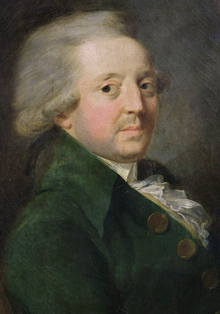
\includegraphics[width=4cm]{Figures/condorcet.png} \\
Marquis de Condorcet
\end{center}
\end{frame}

\begin{frame}
Let $X=\{x_1,x_2,\ldots,x_n\}$ be a finite set of objects to be
ranked.  

Let $a_{ij}$ express the numerical preference between $x_i$
and $x_j$.  
The idea is that $a_{ij}$ estimates ``how much better''
$x_i$ is compared to $x_j$.  

Clearly, for all $i,j$, $a_{ij}>0$ and
$a_{ij}=1/a_{ji}$.  

The intuition is that if $a_{ij}>1$, then $x_i$ is
preferred over $x_j$ by that factor. 

So, for example, Apple's Retina
display has four times the resolution of the Thunderbolt display, and
so if $x_1$ is Retina, and $x_2$ is Thunderbolt, we could say that the
image quality of $x_1$ is four times better than the image quality of
$x_2$, and so $a_{12}=4$, and $a_{21}=1/4$. 

The assignment of values
to the $a_{ij}$'s are often done subjectively by human judges.
\end{frame}

\begin{frame}
Let $A=[a_{ij}]$ be a {\em pairwise comparison matrix}, also known as
a {\em preference matrix}. 

We say that a pairwise comparison matrix is
{\em consistent} if for all $i,j,k$ we have that $a_{ij}a_{jk}=a_{ik}$.
Otherwise, it is {\em inconsistent}.
\end{frame}

\begin{frame}
In practice, the subjective evaluations $a_{ij}$ are seldom
consistent, which creates four problems, and to
this day there is no satisfactory solution to these problems:
\begin{enumerate}
\item How to measure inconsistency and what level is acceptable?
\item How to remove inconsistencies, or lower them to an acceptable
level?
\item How to derive the values $w_i$ starting with an inconsistent
ranking $A$?
\item\label{enum:justify} How to justify a certain method for removing
inconsistencies?  
\end{enumerate}
In real world cases, it is item~\ref{enum:justify}.\ were the
subjective side of the judgments comes most to the fore, as the
``subjectiveness'' of the referees is reflected in the inconsistency
of the resulting matrix.

\end{frame}

\end{document}
